\uuid{JnBb}
\exo7id{7081}
\auteur{megy}
\organisation{exo7}
\datecreate{2017-01-21}
\isIndication{true}
\isCorrection{true}
\chapitre{Géométrie affine euclidienne}
\sousChapitre{Géométrie affine euclidienne du plan}

\contenu{
\texte{
%tags : isocèle, trapèze, symétrie centrale, projection
Soit $\mathcal D$ une droite, $A$ et $B$ deux points hors de cette droite, et $A'$, $B'$ leurs projetés orthogonaux sur $\mathcal D$, supposés distincts. Soit enfin $I$ le milieu de $[AB]$. Montrer que $A'IB'$ est isocèle en $I$.
\begin{center}
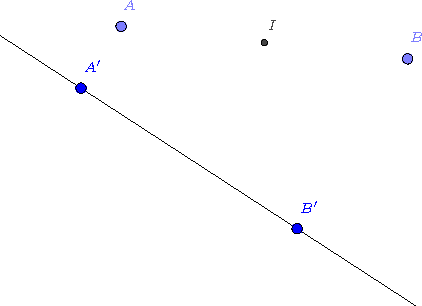
\includegraphics{../images/img007081-1}
\end{center}
}
\indication{De la même façon qu'il est souvent utile de compléter un triangle rectangle en un rectangle, il est souvent utile de compléter un trapèze rectangle en un rectangle.}
\reponse{
On complète le trapèze rectangle $ABB'A'$ en un rectangle comme conseillé, en utiisant la symétrie de centre $I$. 
\begin{center}
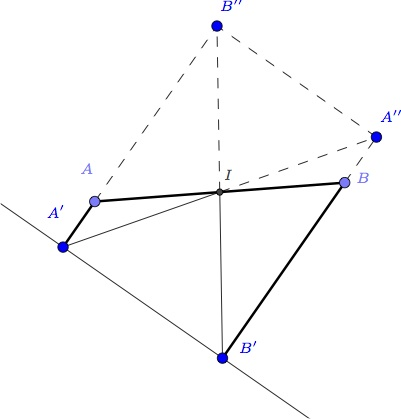
\includegraphics{../images/img007081-2}
\end{center}
Le résultat demandé est alors une conséquence du fait que les diagonales d'un rectangle sont égales et se coupent en leur milieu. 

%On peut aussi utiliser le théorème des milieux.
}
}
